\clearemptydoublepage

\chapter{Les émotions dans la parole}

 \section{Définition de l'émotion}
L'étude de l'émotion humaine est à la croisée de plusieurs domaines dont notamment la psychologie, la physiologie et la linguistique. Sa définition et sa caractérisation est encore aujourd'hui source d'études. En effet, il n'y a pas de consensus clair et établie sur une définition et une théorie qui prime sur les autres.

La définition de l'émotion est exprimée différemment en fonction des domaines d'étude. Pour le grand public, le dictionnaire Le Robert (www.shorturl.at/dsyNV) définit trois sens du mot émotion :
\begin{itemize}
    \item État affectif intense, caractérisé par des troubles divers (pâleur, accélération du pouls, etc.). Par exemple : Être paralysé par l'émotion ; Tu nous as donné des émotions, tu nous as fait peur (familier).
    \item État affectif, plaisir ou douleur, nettement prononcé.
    \item Sensibilité. Par exemple : Interpréter une œuvre avec émotion.
\end{itemize}
Au sein de cette thèse, nous considérons l'émotion selon la deuxième définition : l'émotion est un état temporaire dans lequel se trouve une personne, causée par un sentiment vif ressenti habituellement en réponse à une stimulation de l'environnement.

\subsection{Frise historique des théories de l'émotion}

\begin{figure}
  \centering
  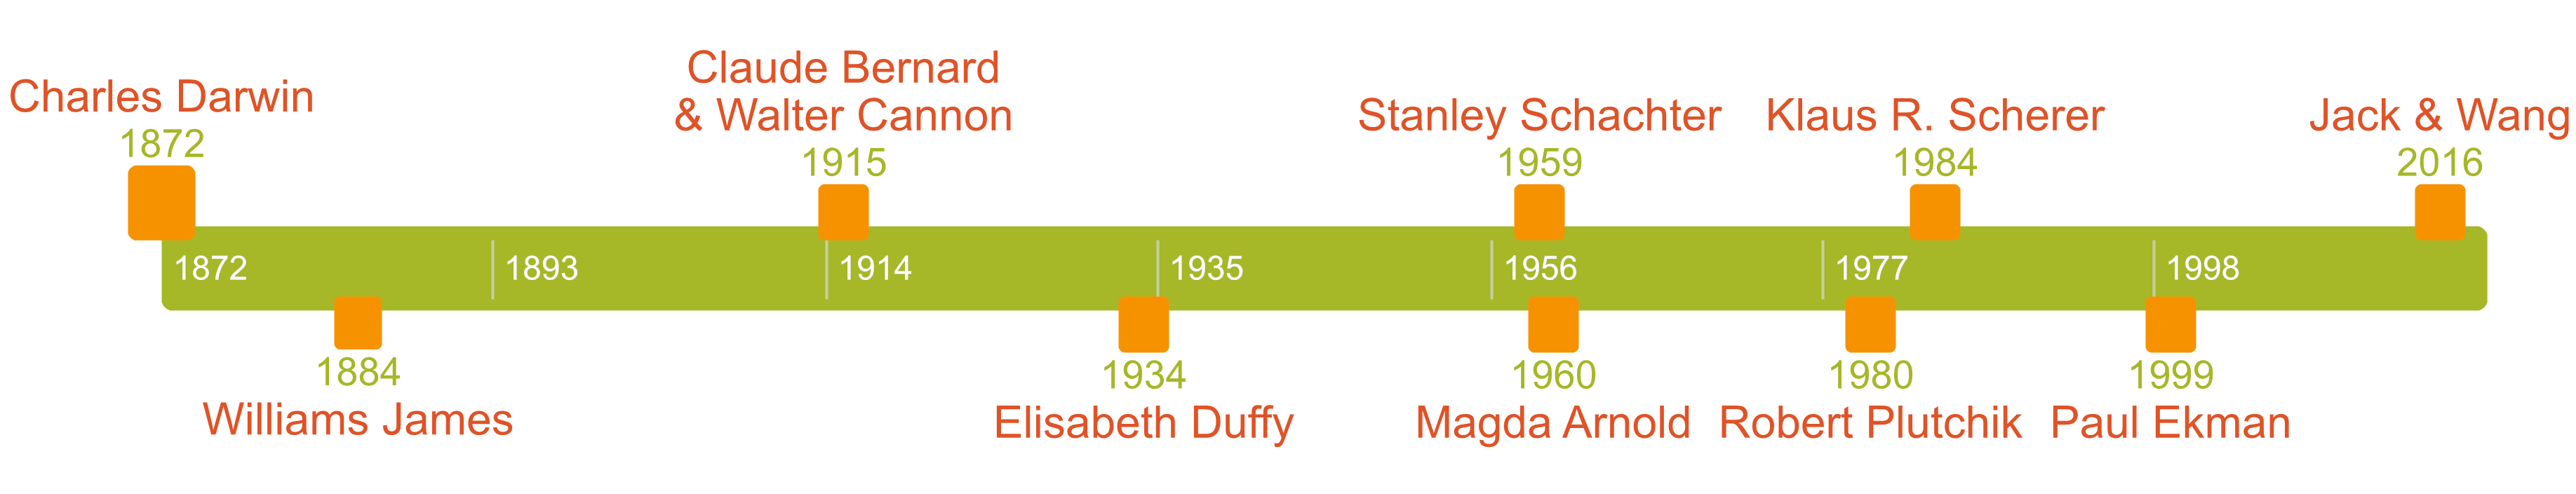
\includegraphics[width=16cm]{./Chapitre1/figures/friseHisto.png}
  \caption{Frise chronologique des grandes théories des émotions selon leur première date de parution}
  \label{fig:Circumplex}
\end{figure}


L'émotion et les états emotionnels, non content de ne pas avoir une unique définition, ont évolués dans leur caractérisation au fil du temps. Les premières mentions scientifiques de l'émotion nous viennent d'Aristote qui, au 4e siècle, définit l'Être comme une combinaison d'émotion et de raison. Bien plus tard, au 16e siècle, d'autres philosophes se sont intéressés à l'émotion tout en le mettant en relation avec la raison. Spinoza théorisait que les états émotionnels avaient une influence sur le raisonnement humain, tandis que Descartes pensait que ces deux notions étaient décorélées.
L'étude contemporaire des états émotionnels a réellement débuté avec les travaux de Darwin (1872), qui a définit les septs principes régissant l'émotion:
\begin{itemize}
    \item les émotion sont innées : elles sont dues à l'Évolution et présentes dès la naissance. Elles se complexifient lorsque la personne grandit.
    \item elles suivent une continuité phylogénétique : les émotions sont aussi présentes chez les animaux proches de l'être humain, par exemple les primates.
    \item les émotions sont dénombrables : on peut caractériser chaque émotion par une des 8 catégories définies par Darwin (souffrances, abattement, joie, mauvaise humeur, haine, mépris, surprise et honte).
    \item elles sont analysables : on peut les caractériser en fonction de l'activité musculaire du visage.
    \item les émotions sont reconnaissables : les témoins reconnaissent l'émotion d'une personne en tant qu'information.
    \item elles sont universelles : comme elles viennent de l'Évolution, elles sont multi-culturelles et leur manifestation est reconnaissable par tous.
    \item elles sont actionnables : "le simple acte de simuler une expression tend à la faire naître dans notre esprit".
\end{itemize}
Les émotions servent donc à la survie de l’espèce et sont définies comme adaptatives. En effet, elles permettent d'adopter une réaction appropriée à un stimuli de l'environnement. Par exemple un danger se présente, concrètement un hippopotame. L'homme ressent une émotion en réponse à ce stimuli : la peur. Celle ci va activer toute une chaîne de réponses biologiques pour augmenter les chances de survie, notamment l'augmentation du rythme cardiaque pour mieux oxygéner les muscles et qui va permettre à l'homme de mieux attaquer ou fuir. \\
Avec la naissance de la psychologie, de nombreuses théories ont émergées pour définir et caractériser l'émotion. Williams James (1884) définit lui l'émotion comme une conséquence de la réponse physiologique à un stimuli de l'environnement. Si une personne nous insulte, on ne crie pas parce qu'on est en colère, on est en colère parce qu'on crie. Cela implique que les émotions sont plutôt contrôlables, on peut les accentuer ou les inhiber.
Dans le cadre des travaux de Claude Bernard et Walter Cannon (1915, 1927), la notion d’homéostasie est définie: l'émotion est un processus qui permet au corps d'interrompre son fonctionnement normal pour concentrer ses ressources dans une réponse adaptée, principalement l'attaque ou la fuite avec notamment la libération d'adrénaline dans le corps. Ces travaux lui permettront également de situer la partie du cerveau responsable de l'émotion : les régions sous-corticales.
Les conclusions de ces travaux lanceront l'exploration du cerveau pour trouver les régions responsables des différentes émotions, amenant les neurosciences à s'emparer du domaine de l'émotion. \\
En parallèle de ces explorations, la notion d'activation va émerger avec Élisabeth Duffy (1934, 1941). En effet, maintenant que les émotions sont détectables dans le cerveau humain, elles vont être traduites par des mesures du potentiel d'activité. La théorie des émotions en catégories comme définie par Darwin est donc réévaluée. En effet, si toutes les émotions peuvent être mesurées en potentiel d'activité de certaines zones du cerveau, la frontière entre les émotions peut être plus perméable que préalablement définie. \\
Cette notion sera néanmoins plus difficile à démontrer que prévu, puisque les époux Lacey (1958) ont constaté que toutes les mesures (électro-encéphalogramme, activité des viscères, tension musculaires) ne covarie pas et sont différentes d'un individu à un autre. \\
Suite à ce revers, Stanley Schachter (1959) a proposé sa théorie cognitivo-physiologique. Selon lui, nous définissons nos émotions en fonction de la situation dans laquelle nous nous trouvons. En effet, nous devons raisonner pour définir nos propres émotions, en \textit{attribuant} celle-ci à un contexte interne ou externe. L'émotion nait donc de deux facteurs : l'activation physiologique et l'attribution cognitive. L'état émotionnel n'est donc plus une simple réponse à un stimulis de l'environnement, elle implique également une part de raisonnement. \\
En s'appuyant sur ces travaux, Magda Arnold (1960) va amorcer la théorie de l'évaluation, qui va prendre de l'ampleur avec les travaux de Scherer (1984). Ce dernier considère que l'évaluation d'une situation est définie par 5 questionnements :
\begin{itemize}
  \item Est-ce que la situation est nouvelle ? (nouvelle/ancienne)
  \item Est-ce qu'elle suscite du plaisir intrinsèque ? (agréable/désagréable)
  \item Est-ce qu'elle est pertinente ? (aidante/génante)
  \item Est-ce qu'on sait y faire face ? (on a le controle/ on n'a pas le controle)
  \item Est-ce que c'est compatible avec les normes ? (compatible avec les normes sociales et ses propres convictions)
\end{itemize}
C'est en réponse à ces 5 questions que Scherer va proposer 5 dimensions pour représenter l'émotion : la nouveauté, la valence, le rapport aux buts, le potentiel de maitrise et l'accord avec les normes. La grille d'évaluation, présentée dans le tableau~\ref{tab:Scherer}, permet de caractériser l'état émotionnel d'un individu en 4 émotions : la colère/rage, la peur, la tristesse et la joie. C'est à partir de ces études que le domaine de l'informatique va se mettre au service de l'étude de l'émotion.

\begin{table}[]
\begin{tabular}{|l|l|l|l|l|}
\hline
\multicolumn{1}{|c|}{\textbf{Dimension d’évaluation}} & \multicolumn{1}{c|}{\multirow{2}{*}{\textbf{Colère/Rage}}} & \multicolumn{1}{c|}{\multirow{2}{*}{\textbf{Peur}}} & \multicolumn{1}{c|}{\multirow{2}{*}{\textbf{Tristesse}}} & \multicolumn{1}{c|}{\multirow{2}{*}{\textbf{Joie}}} \\
\multicolumn{1}{|c|}{\textbf{émotionnelle}}           & \multicolumn{1}{c|}{}                                      & \multicolumn{1}{c|}{}                               & \multicolumn{1}{c|}{}                                    & \multicolumn{1}{c|}{}                               \\ \hline
\multicolumn{5}{|c|}{\textbf{Nouveauté}}                                                                                                                                                                                                                                                  \\ \hline
Soudaineté                                            & haut                                                       & haut                                                & bas                                                      & bas                                                 \\ \hline
Familiarité                                           & bas                                                        & bas                                                 & bas                                                      & ouvert                                              \\ \hline
Prévisibilité                                         & bas                                                        & bas                                                 & ouvert                                                   & moyen                                               \\ \hline
\multicolumn{5}{|c|}{\textbf{Valence}}                                                                                                                                                                                                                                                    \\ \hline
intrinsèque                                           & ouvert                                                     & bas                                                 & ouvert                                                   & haut                                                \\ \hline
\multicolumn{5}{|c|}{\textbf{Rapport aux buts/besoins}}                                                                                                                                                                                                                                   \\ \hline
Pertinence                                            & haut                                                       & haut                                                & haut                                                     & moyen                                               \\ \hline
Degré de certitude dans la                            & \multirow{2}{*}{très haut}                                 & \multirow{2}{*}{haut}                               & \multirow{2}{*}{très haut}                               & \multirow{2}{*}{très haut}                          \\
prédiction des conséquences                           &                                                            &                                                     &                                                          &                                                     \\ \hline
Congruence avec les attentes                          & dissonant                                                  & dissonant                                           & ouvert                                                   & consonnant                                          \\ \hline
Opportunité                                           & obstruction                                                & obstruction                                         & obstruction                                              & facilitation                                        \\ \hline
Urgence                                               & haut                                                       & très haut                                           & bas                                                      & très bas                                            \\ \hline
\multicolumn{5}{|c|}{\textbf{Potentiel de maîtrise}}                                                                                                                                                                                                                                      \\ \hline
Causalité : agent                                     & autrui                                                     & autrui/naturel                                      & ouvert                                                   & ouvert                                              \\ \hline
Causalité : motivation                                & intentionnel                                               & ouvert                                              & hasard                                                   & intentionne                                         \\ \hline
Contrôle                                              & haut                                                       & ouvert                                              & très bas                                                 & ouvert                                              \\ \hline
Puissance                                             & haut                                                       & très bas                                            & très bas                                                 & ouvert                                              \\ \hline
Ajustement                                            & haut                                                       & bas                                                 & moyen                                                    & haut                                                \\ \hline
\multicolumn{5}{|c|}{\textbf{Accord avec les normes}}                                                                                                                                                                                                                                     \\ \hline
Standards externes                                    & ouvert                                                     & ouvert                                              & ouvert                                                   & ouvert                                              \\ \hline
Standards internes                                    & bas                                                        & ouvert                                              & ouvert                                                   & ouvert                                              \\ \hline
\end{tabular}
\label{tab:Scherer}
\caption{Grille d'évaluation des premiers travaux de Scherer pour définir une émotion en fonction des 5 questionnements. In P. Philippot. (2007). Emotion et psychothérapie (pp.11-64). La catégorie ouvert est utilisé lorsque l'évaluation peut etre de différente catégorie. Par exemple, pour la joie, l'élément déclencheur peut être quelque chose de connu ou non (Familiarité). En rapport aux buts/besoins, les opportunités peuvent être obstruées (émotions négatives) ou facilitées (émotions positives).}
\end{table}


\section{Représentation courante des émotions à but d'automatisation de traitement}
Comme nous l'avons vu précédemment, il n'y a pas de consensus sur une définition ou même une caractérisation des états émotionnels. Cela peut être expliqué par notamment, la multitude de domaines qui sont intéréssées par l'émotion (psychologie, physiologie, linguistique, phonologie, sciences cognitives, informatique...) ou encore la part non négligeable de subjectivité du domaine.
Néanmoins dans le domaine de l'informatique, nous faisons principalement la distinction entre deux grands courants de théorie : l'émotion définit par des états discrets et/ou par des états continus. En effet, afin d'automatisation le traitement des émotions, il est nécessaire de se tenir à une théorie algoriquement descriptive, et donc de définir des représentations de l'émotion qui soient en adéquation avec les besoins exprimées par la tache à réaliser, ici la détection et la caractérisation automatique d'émotions contenus dans la parole. Nous proposons donc de rappeler la définition de ces deux ensembles de théorie qui sont "dans une guerre centenaire" l'une contre l'autre, donnant naissance à la multitude de définition que nous lui connaissons.

\subsection{Théorie des émotions discrètes}
La théorie des émotions discrètes considère qu'il existe un nombre illimitée d'émotions qui peuvent être formellement caractérisées. Certaines d'entre elles sont définies comme étant "basiques" ou "primaires" et permettent, en se combinant, d'exprimer des émotions plus "complexes". Darwin est l'un des premiers à définir ces émotions basiques, au nombre de 5 (la colère, la peur, la tristesse, le dégout et la joie), dans sa théorie de l'évolution où il explique que les émotions sont nécessaires à la survie de l'homme, ce qui expliquerait notamment pourquoi elles ont une influence sur notre biologie, nous permettant également de les reconnaitre.
Comme a dit Izard : "people need the category label of fear to explain flight to one another for safety, anger to explain the frustration of blocked goal responses, joy (or its equivalent) to explain the pride of achievement, and sadness to explain the experience of a life-changing loss"~\cite{Izard2007}.
Cependant il n'y a pas de théorie principale qui permettrait de définir ces émotions basiques, de les dénombrer ou d'expliquer leur combinaison en émotions complexes. D'autant plus que les émotions et leur manifestation n'ont pas cessé d'évoluer en fonction des évolutions de nos sociétés.

\begin{table}[]
\begin{tabular}{|l|l|}
\hline
\textbf{Auteyrs} & \textbf{Émotions basiques} \\ \hline
Darwin (1872)       & colère, peur, joie, tristesse, dégoût                                                               \\ \hline
James (1884)        & peur, douleur/chagrin, amour, rage                                                                  \\ \hline
Arnold (1960)       & \begin{tabular}[c]{@{}l@{}} colère, aversion, haine, peur, découragement, \\
                              courage, amour, désir, espoir, désespoir, tristesse\end{tabular}                            \\ \hline
Tomkins (1962)      & rage, peur, joie, angoisse, dégoût, surprise , intérêt, honte                                      \\ \hline
Izard (1971)        & \begin{tabular}[c]{@{}l@{}} intérêt, joie, surprise, tristesse, colère, dégoût, mépris, \\
                              auto-hostilité, peur, honte, timidité, culpabilité \end{tabular}                            \\ \hline
Plutchik (1980)     & \begin{tabular}[c]{@{}l@{}} colère, peur, joie, tristesse, dégoût, surprise,  \\
                              acceptation, anticipation \end{tabular}                                                     \\ \hline
Frijda (1986)       & désir, intérêt, bonheur, surprise                                                                   \\ \hline
Oatley \& Jonhson-Laird (1987)    & colère, dégoût, inquiétude, bonheur, tristesse                                        \\ \hline
Gray (1990)         & rage, terreur, anxiété, joie                                                                        \\ \hline
Ekman (1999)        & colère, peur, joie, tristesse, dégoût, surprise                                                     \\ \hline
\begin{tabular}[c]{@{}l@{}}Jack (2016), Gu (2015)
  \\ et Wang (2016)\end{tabular}   & peur, colère, joie, tristesse                                                        \\ \hline
\end{tabular}
\label{tab:EmotionsBasiques}
\caption{Définition des émotions basiques selon différents auteurs}
\end{table}


De nombreux auteurs ont proposés des émotions primaires : Ekman propose 6 émotions basiques (la peur, la colère, la joie, la tristesse, le dégout et la surprise) qu'on appelera par la suite les "Big Six", tandis que Plutchik en propose 8 (la colère, la peur, la tristesse, le dégout, la surprise, l'anticipation, la confiance et la joie). Jack, Gu et Wang ont quand à eux proposés 4 émotions basiques (la peur, la colère, la joie et la tristesse). Le tableau~\ref{tab:EmotionsBasiques} liste, en partie, les définitions des émotions primaires selon leurs auteurs. Toutes ces caractérisations sont souvent définies en fonction d'un contexte d'étude, d'un but à atteindre.

\begin{figure}
  \centering
  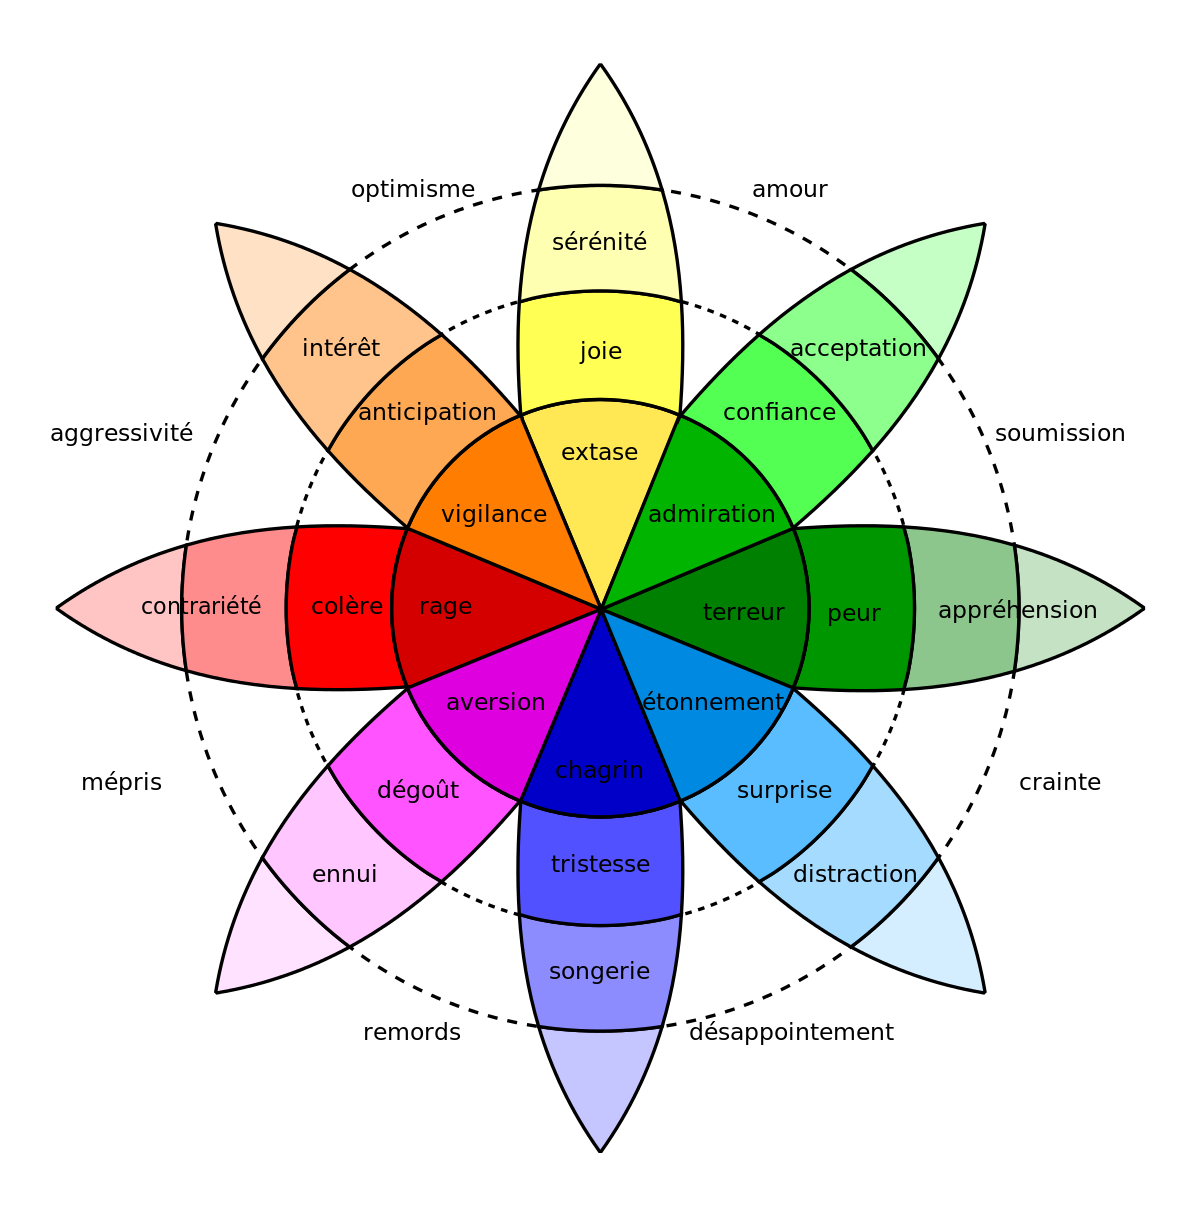
\includegraphics[width=12cm]{./Chapitre1/figures/Plutchik.png}
  \caption{Roue de Plutchik qui définit les émotions complexes à partir d'émotions basiques.}
  \label{fig:Plutchik}
\end{figure}


Ces émotions primaires peuvent également se combiner pour donner des émotions dites "complexes", qui permettent de nuancer les états émotionnels. C'est notamment le cas avec la roue de Plutchik, présentée dans la figure~\ref{fig:Plutchik}, qui dénombre 32 émotions caractérisées en 8 émotions primaires selon leur intensité. De plus, on parle également d'émotions secondaires afin de décrire des émotions qui ne sont pas innées, mais qui sont apprises pendant le développement de la personne. Ekman définit ainsi 9 émotions secondaires, plus complexes et plus difficiles à identifier (la culpabilité, l'embarras, le mépris, la complaisance, l'enthousiasme, la fierté, le plaisir, la satisfaction et la honte) qui sont marquent des différences d'expression en fonction des cultures et des individus. Charland (1995) et Damasio (1994) ont notamment contribués à analyser les différences culturelles de ces émotions secondaires.
En plus de ces théories discrètes, l'émotion peut être définie par de nombreuses théories continues.

\subsection{Théorie des émotions continues}

\begin{figure}
  \centering
  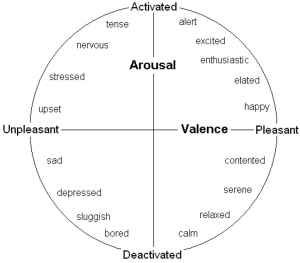
\includegraphics[width=8cm]{./Chapitre1/figures/Circumplex.png}
  \caption{Le modèle circumplex de Russell}
  \label{fig:Circumplex}
\end{figure}

Une autre façon de définir les émotions est de les inscrire dans des espaces continus. La théorie des émotions continues, aussi appelée émotions en dimensions, a été introduit par les travaux de Wundt (1902) et Schlosberg (1954). Les émotions sont descriptibles selons trois dimensions indépendantes nommées en fonction de leur extremum : agréable-désagréable, tendu-détendu et agité-calme. Grace à ces trois dimensions, chaque émotion ressentie par un individu peut être décrite comme une combinaison pondérée de ces trois axes. Comme ces dimensions se chevauchaient, ces dernières ont été remplacées par le modèle du circumplex, présentée dans la figure~\ref{fig:Circumplex} de Russell en 1980, devenant la théorie principale permettant de décrire les émotions de façon continue. Ce modèle permet de placer toutes les émotions au sein d'un cercle dont l'abscisse définit la valence de l'émotion (positive-négative) et l'ordonnée définit l'activation (faible-fort). D'autres axes ont également été ajoutées sur ce modèle par Scherer (2005) comme la dominance, l'intention ou l'axe conducteur/obstructif, comme illustré dans la figure~\ref{fig:Genova}. Par exemple, on peut voir que la mélancholie (melancholic) a une valence neutre et une faible activation, tandis que la deception (disappointed) a une valence très négative et une activation neutre.
\begin{figure}
  \centering
  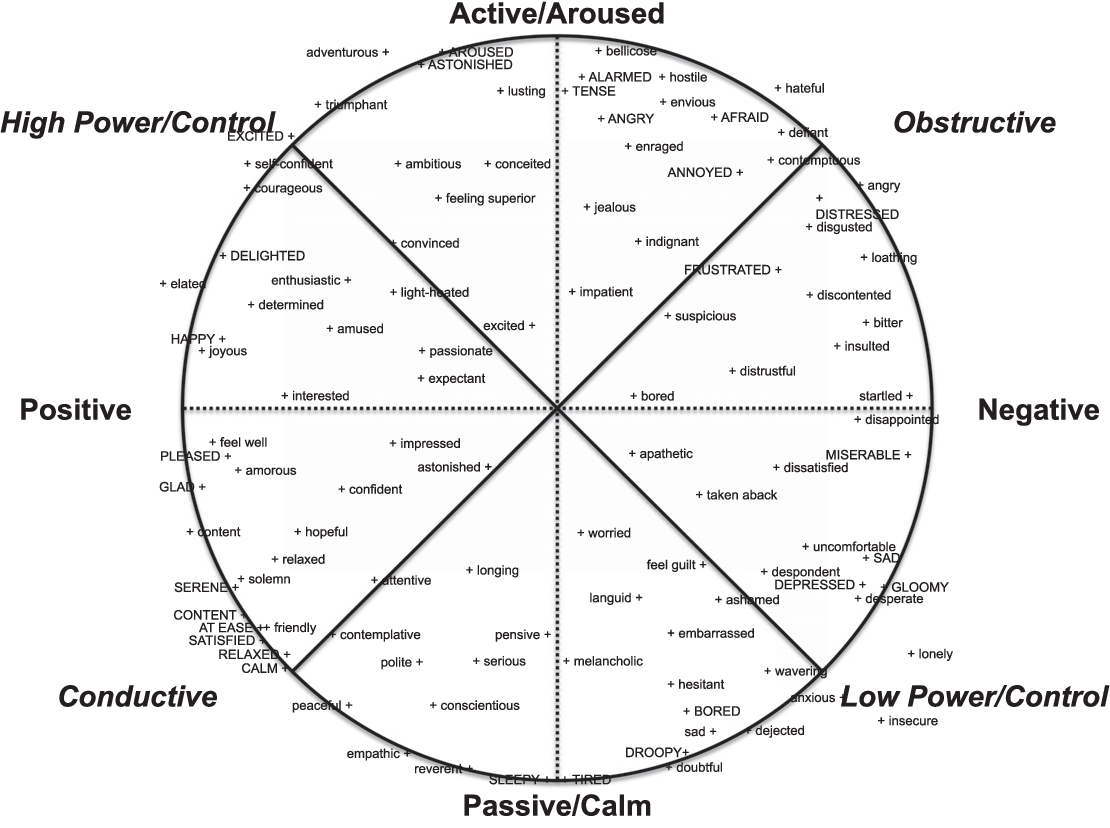
\includegraphics[width=18cm]{./Chapitre1/figures/Genova.png}
  \caption{La roue des émotions de Genève définie par Scherer, qui nomme des émotions (primaires ou secondaires) dans des dimensions continues.}
  \label{fig:Genova}
\end{figure}

Un système à trois dimensions, jugeant en plus de l'engagement de l'émotion, a également été concu. Mais il est peu utilisé en informatique car il apportait que peu d'information pour une forte complexité, ne permettant de mettre faciement en place des systèmes d'annotation par exemple.
Ces dimensions peuvent être discrétisées par des systèmes de graduations, permettant notamment de faire le lien avec des théories discrètes.
En ce qui concerne les études menées sur les émotions continues dans le domaine de l'informatique, il y a une forte prévalence des dimensions de valence et d'activation quelque soit le support utilisé (la voix, le texte, la vidéo ou des données physiologiques).
Au sein de cette thèse, nous avons décidé de nous appuyer sur la théorie des émotions continues, afin de répondre à la problématique industrielle.


\section{L'émotion dans la parole : para-linguistique et prosodie}
Si nous nous replaçons dans le contexte de cette thèse, notre objectif est de décrire l'émotion humaine lors de conversations tenues entre un client et un agent dans un cadre défini par un appel téléphonique en centre d'appels. Nous n'avons donc que la voix comme axe d'analyse pour en retirer les états émotionnels des intervenants.
La voix que l'on considère comme un canal de communication comme définit par Shannon (1948), permet de faire passer un message entre un émetteur (ici le locuteur) et un récepteur (ici l'écoutant). Les informations communiquées par ce biais peuvent être divisées en deux catégories, la linguistique et le para-linguistique.
Le linguistique va décrit le language en tant que parole de base tandis que le para-linguistique va définit tout ce qui n'est pas du message verbal. Par exemple, dans la vie de tous les jours, "Bonjour, je voudrais une baguette de pain" correspond au message linguistique, tandis que le sourire, le geste de la main, l'hésitation vocale ou le raclement de gorge fera partie du domaine para-linguistique. Shirley Weitz (1974) explique que la paralinguistique s'intéresse "à la façon dont quelque chose est dit, pas à ce qui est dit". Globalement, on considère du domaine du para-linguistique dans la parole, l'accent, la hauteur, le volume, la vitesse de parole, la modulation, la prosodie et la fluidité de l'élocution.
La définition du paralangage étant évolutive, il est donc naturellement que sa définition reste imprécise comme l'indique Peter Matthews dans ses travaux.
La prosodie est définit par l'ensemble des phénomènes qui accompagnent le discours, tout en n'étant pas du discours. Elle est notamment marquée par trois paramètres très important:
\begin{itemize}
  \item La fréquence fondamentale (fo) de la parole correspond à l'inverse de la période d'un son périodique, c'est à dire à la durée des sons de type voyelles dans la parole.
  \item La durée de la parole
  \item l'intensité de la parole qui est définit par l'énergie contenue dans le signal.
\end{itemize}
C'est par l'étude para-linguistique et notamment l'étude de la prosodie que nous analysons inconsciemment le discours d'un locuteur afin de déterminer son état émotionnel.

\section{La présence de marqueurs émotionnels dans le texte}
